\chapter{Background theory}
Before we move to the nuts and bolts of AlphaZero and our concrete implementation for Abalone, we should establish a general understanding of the problem. That includes building the necessary theoretical background in artificial intelligence in general, as well as insight into the specialized knowledge such as deep reinforcement learning in particular.

\section{Artificial intelligence}
The introduction has already forshadowed how the field of artificial intelligence has undergone a shift in their methodology. In the 1950s and 1960s figures like Alan Turing and von Neumann laid the foundations for modern computers. This sparked the idea one could create programs for these new machines that have similar abilities like humans and other organisms. Researchers at that time assumed there is no "universal principle" behind intelligence and focused on reason and symbol manipulation. Therefore these methods were considered "strong techniques", methods that relied on general principles like learning were labeled "weak techniques". Nowadays, the consensus in the field has revesered. \cite[p. 8f.]{sutton_reinforcement_2018}

\subsection{Rational agent}
Stemming from the latin word \textit{agere} meaning "to act", an agent is something that acts. As we expect an agent to take sensible or intelligent actions we further qualify this definition by calling it rational. This means that it acts so as "to achieve the best outcome or, when there is uncertainty, the best expected outcome". \cite[p. 36]{russell_artificial_2021}

The agent exists in an environment which it perceives through sensors and it takes actions through its actuators. We refer to the content of the sensor's output for one observation as \textit{percept}. A cat uses eyes, ears and other organs to perceive the world and its legs, claws and so on to interact with the world. An autonomous car might use radar and cameras for acquiring information and steering and motors for navigation.

Internally the agent might have some built-in knowledge about the world, such as rules on how the environment works. The \textit{agent function} takes the entire history of percepts observed and this built-in knowledge and maps it to an action. A concrete implementation of this abstract function is called \textit{agent program}. The agent program might just be a simple tabular mapping from percepts to actions or could use a complex algorithm with an additional model.

\subsection{(Task) environment}
\label{environment}

As we are trying to build an agent that tries to achieve some specified goal, we can consider its environment as a problem or \textit{task} the agent tries to solve. Putting together both agent and the environment we see a loop of observing,  deliberating and finally taking an action as depicted in figure \ref{agent_environment_loop}.

\begin{figure}
    \centering
    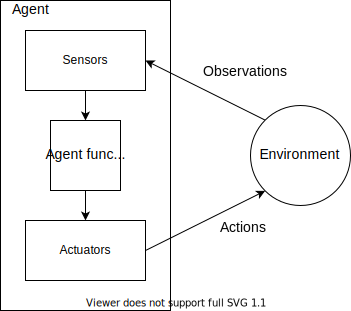
\includegraphics[height=7cm, keepaspectratio]{agent_environment_loop.png}
    \caption{The agent-environment interaction loop \cite[cf. p. 96]{russell_artificial_2021}}
    \label{agent_environment_loop}
\end{figure}

To specify the task environment there are four key components. Let us specify the task environment for a machine classifying defective parts in a production line:

\begin{enumerate}
    \item Performance measure: This might be the percentage of correctly broken parts (true positives) weighted against the number of incorrectly identified parts (false positives).
    \item Environment: The conveyor belt and the parts
    \item Actuators: An arm to push the parts to a different conveyor belt
    \item Sensors: Possibly a camera, infrared sensors, etc.
\end{enumerate}

The initial letters form the acronym PEAS (framework).

There are a few categorizations of the properties of task environments that are extremely helpful for narrowing down potential applicability of different classes of algorithms. A key property is the observability of the environment. If the environment is \textit{fully observable}, the sensors detect all the information that is in any way relevant for taking an action. Conversely if not all information can be observed we call it \textit{partial observability}. For example in poker the other players' cards and the upcoming cards cannot be seen but are highly relevant to the agent's actions. As the current board state of chess fully comprises all information necessary to make a move, we can classify it as fully observable.

The values of the state of the environment and time can be categorized into discrete and continuous. An autonomous vehicle for instance is dealing with continuous time and also continuous states. The speed of the car takes a smooth range of real values and time can be meaningfully split into increasingly small intervals. Board games are entirely discrete. The set of all states is a finite collection of all (legal) permutations of the board and the marbles. Time progresses on the basis of turns.

An agent's actions might also be \textit{non-deterministic}. When dealing with systems of high complexity the next state might not only depend on the previous state and the action taken. There might be other car drivers taking unexpected actions or a comet hitting our car.

Further expanding on the passage of time we have to take into account if actions have consequences for future states. If each combination of percept and action is independent of each other we call it \textit{episodic} and \textit{sequential} otherwise. If we had to classify a production line of circuit boards as either defective or functional, it would be an episodic environment. The classification of an individual board does not matter for the next one.

Another aspect of time is whether the environment changes while the agent takes time to deliberate on the next move. In a \textit{dynamic} environment like the autonomous vehicle operates in, the environment changes continuously. By the time the car decides whether to go right, to avoid collision with a wall, this decision might have already become obsolete. A  turn-based game like chess is static as the board only changes when a move is made.

Lastly, an additional dimension to consider is the number of agents involved. The classification of circuit boards only involves one agent whereas chess is a \textit{multi-agent} environment. We also have to distinguish whether those multiple agents compete for the performance measure. In most board games, one player's win is the other player's loss. In contrast, the other vehicles apart from our autonomous vehicle all profit when it avoids a collision and vice versa. Therefore, they cooperate.



\section{Classic agent}
Now that we have an intricate understanding of the environment of agents we have also narrowed down the choice of algorithms we can employ. In general, perfect information games can be solved by adversarial search algorithms. That means in theory one can find the optimal solution by traversing the entire game tree to terminal states (game ending state). The theory behind this type of agent was already laid out as early as 1945 by Konrad Zuse's program generating legal chess moves \cite{knuth_early_1980}, but was described most comprehensively by Claude Shannon in 1950 in "Programming a Computer for Playing Chess". \cite{shannon_xxii_1950}

\subsection{Minimax algorithm}
Minimax assumes two roles: The minimizer ($min$) and the maximizer ($max$). We start the search from the current board state as the role of the maximizer and then alternate between the two. The result of the minimax search gives us the maximum utility for the given state, assuming both players behave optimally. Let us define the functions \cite[p. 303f.]{russell_artificial_2021}
\begin{itemize}
    \item $\texttt{utility}(s, p)$ returns the utility or the payoff for the terminal state $s$ seen from the perspective of player $p$. In the case of chess this might be $-1, 0$ and $1$ for a loss, draw and a win.
    \item $\texttt{is-terminal}(s)$ returns whether the given state $s$ is a terminal state or not.
    \item $\texttt{to-move}(s)$ returns the current player for the state $s$, either $min$ or $max$.
    \item $\texttt{result}(s, a)$ returns the resulting state if in state $s$ and taking action $a$.
    \item $\texttt{actions}(s)$ returns all legal moves for the given state $s$.
\end{itemize}

\begin{equation}
    \texttt{minimax}(s) =
    \begin{cases}
        \texttt{utility}(s, max)                                                      & \texttt{is-terminal}(s)    \\
        \texttt{max}_{a\in\texttt{actions}(s)}\texttt{minimax}(\texttt{result}(s, a)) & \texttt{to-move}(s) == max \\
        \texttt{min}_{a\in\texttt{actions}(s)}\texttt{minimax}(\texttt{result}(s, a)) & \texttt{to-move}(s) == min \\
    \end{cases}
\end{equation}

Putting this together we can see in figure \ref{minimax} a graphical representation of the search tree for an abstract example. The algorithm traverses down to a leaf node, evaluates its utility and passes the value back up to the parent node. Depending on whether it is a minimizer or a maximizer it chooses the smallest or the largest value passed up by its children. This value again is passed up to the parent until we reach the parent node which is always a maximizer, yielding us the maximum utility we can achieve given our opponent plays optimally.

\begin{figure}
    \centering
    % \includesvg[height=7cm]{minimax.svg}
    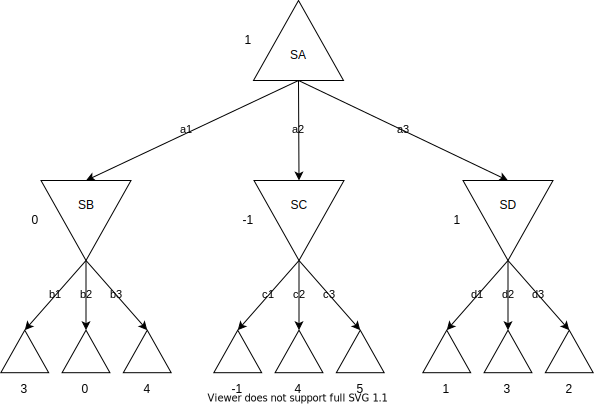
\includegraphics[height=7cm, keepaspectratio]{minimax.png}
    \caption{Minimax for a small search tree, resulting in an utility value of 1}
    \label{minimax}
\end{figure}

\subsection{Heuristic functions}
As the number of nodes of the game tree gets very large, the search on the tree usually does not reach terminal leaves that indicate a clear loss or win. Our computational resources will get exhausted first. For example minimax has already visited $ 361 * 360 * 359 * 358 = 16,702,719,120 $ nodes at a depth of $ d = 4 $ in the case of an average Go game.

Therefore, one has to limit the search to a computationally feasible depth and evaluate the intermediary result of a given transposition based on a so-called \textit{heuristic function}. This function replaces our previous $ utility(s) $ for terminal states and is based on human knowledge. The function should give precise feedback on the quality of a state from the perspective of the given player. A sensible function for chess might be a linear combination in the form of:

$$ h(s) = \omega_0f_0(s) + ... + \omega_nf_n(s) $$

With functions $ f_i $ calculating different values such as

\begin{itemize}
    \item Material: First, we assign an integer to each piece, that represents the piece's relative value (pawn = 1, bishop/knight = 3, rook = 5, and queen = 9). Then sum the values of the pieces left on the board for each player.
    \item Space: Count the squares controlled by each player.
    \item King safety: Check weaknesses in king's position, count attacking piece close to the king etc.
    \item Win and loss: As a more definitive measure we can indicate whether the current state is a terminal state and hence a winning or losing state.
    \item Etc.
\end{itemize}

By applying different weights $ \omega_i $ to the functions $ f_i $ we essentially give incentives to the agent to prioritize certain behavior. If the win or loss function returns a value of either $-1$ or $+1$, we might combine it with a weight of 10,000 to make sure we choose winning states and avoid losing states above all. Armed with this heuristic function we can find good moves with minimax search even in highly complex state spaces.

However, the problem with heuristic functions is we need expert knowledge and a lot of empirical testing to find a suitable heuristic. In some cases like Go, such a heuristic function might not be competitive with even moderate human players. In other cases such as chess this strategy is very powerful. As mentioned in the introduction IBM's Deep Blue could beat the world's best player Gary Kasparov with heuristic based adversarial search.

\subsection{Alpha-beta pruning}
We can further improve minimax search markedly by using Alpha-beta-pruning. This method tries to eliminate unnecessary traversals down the search tree. In the best case, this leads to a reduction of nodes from $ O(b^d) $ to $ O(\sqrt{b^d}) $.

\begin{figure}
    \centering
    % \includesvg[height=7cm]{alpha_beta_pruning.svg}
    \includegraphics[height=7cm, keepaspectratio]{alpha_beta_pruning.png}
    \caption{Our previous example but with alpha beta pruning applied. The grayed out nodes indicate, that these in fact could be pruned from the tree}
    \label{alpha_beta_pruning}
\end{figure}

The order in which we visit nodes in minimax is similar to a graph traversal with depth first search, meaning we descend down until we find a leaf node. This gives us information about the utility of that node and, consequently, part of the tree. Going up the tree we keep an alpha value for the minimum value the maximizer will receive and a beta value for the maximum value the minimizer will achieve. For instance this lets us know if the minimizer already can choose a move worse than what we can achieve with another move, we do not descend further $ (\alpha > \beta) $.

Looking at the example in figure \ref{alpha_beta_pruning} will help us illustrate this principle. Our search revealed that choosing move $ a_1 $ will yield us a utility of at least $0$. Traversing down move $ a_2 $ the first leaf has a utility of $-1$. Hence, the minimizer will choose a move that is at most $-1$ which is already worse than the utility of $0$. We need not look further at this part of the tree.

The example also shows us an important prerequisite for this method to work. The order in which we expand which node matters decides how many nodes we can prune. Had we visited move $ c_3 $ and $ c_2 $ first, pruning wouldn't have been possible. The best case of $ O(\sqrt{b^d}) $ is entirely dependent on this ordering. We could find different ways of ranking the moves:

\begin{itemize}
    \item \textit{Killer move heuristic} prioritizes moves that are usually undoubtedly good like taking a piece in chess.
    \item \textit{Iterative deepening} Performs a minimax search only to a depth of one and uses the resulting values to rank the moves. Then searching one level deeper we use this ranking for ordering the moves. Even though there is a lot of redundancy, we make up for this more than enough by pruning much more effectively.
\end{itemize}

Other improvements to the procedure are thinkable as well. Once we perform a search for a certain state, we can store the resulting utility. If we encounter this position again, because of a different permutation of the move sequence (transposition), we can just look up the state utility in the \textit{transposition table}.

Combined with alpha beta pruning, the minimax algorithm is a very efficient way of finding the optimal utility in an adversarial search situation. However, as mentioned before in most games we cannot use the utility of terminal states, because the search tree grows too quickly. By optimizing for a heuristic function the quality of play solely depends on this function. For games such as chess minimax has been very successful, because humans could devise meaningful heuristic functions. The chess engine stockfish has been the most successful computer player for a long time and is based on this algorithm (and many optimizations). \cite{noauthor_stockfish_2021, noauthor_stockfish_nodate}

\subsection{Monte Carlo Tree Search}
For games like Go we cannot find powerful heuristic functions, which makes the previous approach of minimax not a viable option. In addition, the initial position of a $19\times19$ Go board has a branching factor of $361$ decreasing only by one for each stone placed. A method proposed in 2006 by Coulom \cite{coulom_efficient_2007} called Monte Carlo Tree search was more successful for Go. The main idea is to use simulations or \textit{rollouts (or playouts)} to gain information on the quality of a state. To manage the complexity of the search tree more effectively the algorithm is \textit{selective} in which parts of the tree are \textit{expanded}. This ensures that resources are not wasted on unpromising moves.

In its purest form the simulations are performed randomly, meaning we take a state or node to be investigated and let two random players take turns until a terminal state is reached. Kocsis and Szepesvári \cite{kocsis_bandit_2006} showed that it does in fact converge to optimal play. For games with a high branching factor we need a large number of simulations to get any meaningful information from the simulations, so we might use a \textit{rollout policy} instead. This policy guides the moves taken in the simulation towards better moves. This might be as simple as favoring capturing moves or as we will see later neural networks.

The algorithm iteratively expands the search tree. For each iteration it runs through four steps:
\begin{itemize}
    \item \textbf{Selection} is the process of deciding which node to consider next. We start at the root node and select a node until we reach a leaf node. This is the selected Node. We could select the nodes according to some stationary distribution or we could use the information that we gain over time.

    \item \textbf{Expansion} is the step in which we expand the selected node by appending a fresh child node.

    \item \textbf{Simulation} is as described before the step in which we perform a simulation with our rollout policy starting from the state of the newly generated child node.

    \item \textbf{Back-propagation} is the last step. We take the result of the simulation (utility) and write it to the node and parent nodes above until we reach the root node. Each node updates its cumulative utility $U(n)$ and the number of times it was visited $N(n)$.
\end{itemize}

The more this cycle is repeated, the more certainty is gained about the best move to take.

\begin{figure}
    \centering
    % \includesvg[height=7cm]{minimax.svg}
    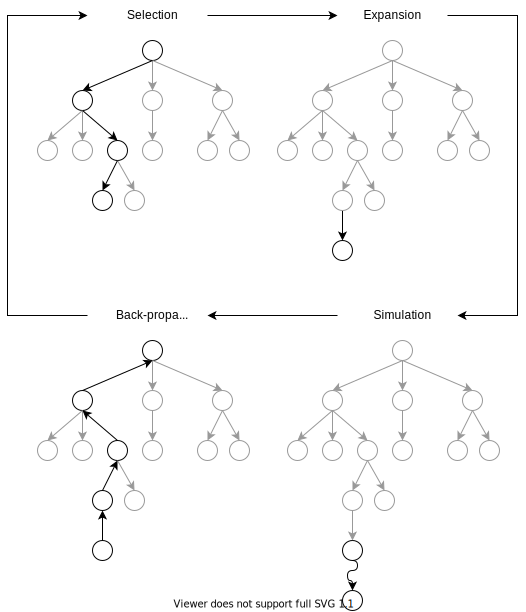
\includegraphics[height=9cm, keepaspectratio]{monte_carlo_tree_search.png}
    \caption{Monte Carlo tree search stages \cite{noauthor_fig_nodate}}
    \label{monte_carlo_tree_search}
\end{figure}

The development of MCTS led to significant improvements in performance of game-playing agents in the game of Go. The algorithm "Crazy Stone" from Coulom won the 10th KGS computer-Go tournament against competitors such as Indigo \cite{bouzy_associating_2006}. To select the next node the program estimates the probability of that move being better than the current best move. Then it orders the moves by their current estimated value $ \mu_i $ and calculates the corresponding variance $ \sigma_{i}^{2} $ getting the ordering of $ \mu_0 > \mu_1 > ... > \mu_N $. Selection of a move is proportional to:

$$
    u_i = exp\left(-2.4\frac{\mu_0 - \mu_i}{\sqrt{2(\sigma_{0}^{2} + \sigma_{i}^{2})}}\right) + \epsilon_i
$$

The Term $ \epsilon_i $ ensures that the probability of selection never goes to zero as defined by $ \epsilon_i = \frac{0.1 + 2^{-i} + a_i}{N} $. The resulting distribution is similar to the Gaussian distribution and the Boltzman equations \cite{coulom_efficient_2007}

Another idea for selection is the UCB1 formula \cite{auer_finite-time_nodate}, that weights how often we have visited a node and how promising it is.

$$
    \text{UCB1}(n) = \frac{U(n)}{N(n)} + C \times \sqrt{\frac{\log{N(Parent(n))}}{N(n)}}
$$

The cumulative utility $U(n)$ is normalized by the number of times we have visited the node $N(u)$. This helps favor moves that are either relatively unexplored and promising or have proven to be good over a larger set of nodes. It is also called the exploitation term. The additional term is called the exploitation term. The more often we visit a node, the smaller this term gets, converging to 0 for large $N(n)$. The constant factor $C$ is subject to some debate which value might be optimal, some choose $\sqrt{2}$. In general, this hints at another point of investigation: The problem of \textit{exploration vs. exploitation} \ref{exploration_vs_exploitation} that we will inspect more closely later.

Here we can already see David Silver's handwriting on the wall. As early as 2006 he, and Sylvian Gelly, investigated optimization to MCTS \cite{gelly_achieving_nodate} for the game of Go. In 2011 they published a comprehensive paper \cite{gelly_monte-carlo_2011} proposing the algorithm MoGo and evaluating different strategies to improve the effectiveness of MCTS in Go. Seeing that

\begin{quotation}
    [...] professional Go players often play moves according to intuitive feelings that are hard to express or quantify. Precisely encoding their knowledge into machine-understandable rules has proven to be a dead-end: a classic example of the knowledge acquisition bottleneck.
\end{quotation}

One of the ideas introduced is Rapid Action Value Estimation (RAVE). We already saw how we could reuse information gathered for minimax through a transposition table. In our search tree we will encounter transpositions for that we already performed searches. RAVE allows us to reuse experience gathered from simulations for related positions. A key property observed by Silver was that MoGo scales proportional to the amount of compute or rather number of simulations it can perform per turn as depicted in figure \ref{mogo_scaling}.

\begin{figure}
    \centering
    \includegraphics[height=7cm, keepaspectratio]{mogo_scaling.png}
    \caption{Elo rating of MoGo in relation to the computational resources granted to the algorithm \cite{gelly_monte-carlo_2011}}
    \label{mogo_scaling}
\end{figure}

\section{Learning agent}
The methods described until this point can be described as "Good old fashioned AI". They rely on search and human knowledge to perform adequately. We shift our focus now to methods that use learning mechanisms to improve their play. With MCTS we've actually seen a kind of intermediary form of algorithm as it is "simulating moves into the future, observing the outcome, and using the outcome to determine which moves are good ones is one kind of reinforcement learning." \cite[p. 331]{russell_artificial_2021}

\subsection{Reinforcement learning}
By devising a heuristic function, we basically told our agent what to do by indicating how a good position looks. The agent optimized its actions to be in a good position as described by the function. In reinforcement learning the agent learns what action to take through interaction. We don't predefine which actions are to be taken. The agent tries to discover which actions yield the best \textit{reward}. The numerical reward signal might come immediately, but e.g. in the case of chess the reward for actions taken comes much later by winning the game (or losing it). According to Sutton and Barto those are the key components of reinforcement learning: "trial-and-error search and delayed reward". \cite[p. 1]{sutton_reinforcement_2018}

Reinforcement learning is not a specific solution or method for this problem domain, all methods for "goal-directed agents interacting in an uncertain environment" \cite[p. 3]{sutton_reinforcement_2018} are types of reinforcement learning. It is a general formalism that will help us reframe the problem of playing a board game (well) in a new light.

\subsection{Markov decision process}
For reinforcement learning we also need to find a formalism for the environment. Originally derived as an extension of Markov Chains by Richard Bellman \cite{yang_markov_2019, bellman_markovian_1957}, the (finite) Markov Decision Process (MDP) describes sequential decision making where actions have long-term consequences, thus, effect future rewards. The MDP is an abstraction of "goal directed learning from abstraction" that reduces the problem to three signals of actions, states and rewards that are being exchanged between the agent and the environment. We already introduced the agent-environment interaction loop in figure \ref{agent_environment_loop}. We can reframe this image with the new terminology of the MDP framework in figure \ref{mdp_agent_environment}.

\begin{figure}
    \centering
    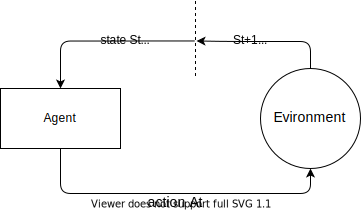
\includegraphics[height=4cm, keepaspectratio]{mdp_agent_environment.png}
    \caption{The markov decision process as agent-environment interaction loop}
    \label{mdp_agent_environment}
\end{figure}

We divide the passage of time into discrete time steps $ t $ at which the agent senses the state $ S_t \in \mathcal{S} $ and then selects some action $ A_t \in \mathcal{A}(s) $. Resulting in that action is some reward $ R_{t+1} \in \mathcal{R} \subset \mathbb{R} $ that is received in the next timestep. For a \textit{finite} MDP the sets $ \mathcal{A}, \mathcal{S}$ and $ \mathcal{R} $ have a finite amount of elements.

The transitions between the state $ s $ and the next state $ s' $ is given by the function $ p $ which essentially defines the decision process as a whole:

$$
    p(s', r | s, a) \doteq Pr\{S_t=s', R_t = r | s_{t-1} = s, A_{t-1}=a\}
$$

As the random variables $ R_t $ and $ S_t $ only depend on the previous state and action, "the state must include information about all aspects of the past agent–environment interaction that make a difference for the future. If it does, then the state is said to have the \textit{Markov property}". \cite[p. 48]{sutton_reinforcement_2018}

From these properties of the MDP we can define the four central components of Reinforcement learning:

\paragraph{The reward signal} is the description of the agent's goal. A controller of a cooling system for a server farm might have the goal to minimize the energy spent for cooling while keeping the servers below a certain threshold. The reward signal then encompasses both of these subgoals. The controller has to maximize this reward. The \textit{reward hypothesis} states that:
\begin{quotation}
    That all of what we mean by goals and purposes can be well thought of as the maximization of the expected value of the cumulative sum of a received scalar signal (called reward).
\end{quotation}
Therefore, we introduce the reward $R_t $ and the goal $ G_t $ which is in the simplest case the sum of future rewards.

$$ G_t = R_{t+1} + R_{t+2} + ... + R_T $$

We might also discount the future rewards by some factor $\gamma \in [0, 1] $ to account for the decrease in certainty we have about future rewards:

$$ G_t = R_{t+1} + \gamma R_{t+2} + \gamma^2 R_{t+2} + ... = \sum_{k=0}^{\infty} \gamma^kR_{t+k+1}$$

\paragraph{The policy} is a mapping between the perceived states to probabilities for selecting each possible action. For TicTacToe we might imagine a table that lists for all possible states to the agent's action. Due to the size of the state space \ref{complexity_table} in more complex games this would not be feasible, therefore we used search processes as a policy so far.

We denote the policy as the function $\pi $ defines a probability distribution over all actions $ a \in \mathcal{A}(s)$ for each $ s \in \mathcal{S} $. $ \pi(a|s)$ is probability at a given timestep $t$ for the action to be $ a = A_t $ under the condition that $ s = S_t $.

\paragraph{The value function} is an estimation of the reward for the agent to be in a given state $ s $.  As the reward for a state depends on what actions we take in the future, the value depends on the policy $ \pi $ defined above. Given that we are at timestep $ t $ and in state $ s = S_t $, the \textit{state-value function $v_{\pi}$}:

$$ v_{\pi}(s) = \mathbb{E}_{\pi}[G_t | S_t = s] = \mathbb{E}_{\pi}\left[\sum_{k=0}^{\infty} \gamma^kR_{t+k+1} \middle| S_t = s \right] $$

The heuristic function entcountered pereviously was essentially a value function being used to guide the game-tree search.

Furthermore, we define the value of action $a$ while being in state $s$ under the policy $pi$ as the \textit{action-value function} $q$:

$$ q_{\pi}(s) = \mathbb{E}_{\pi}[G_t | S_t = s, A_t = a] = \mathbb{E}_{\pi}\left[\sum_{k=0}^{\infty} \gamma^kR_{t+k+1} \middle| S_t = s, A_t = a \right] $$

\begin{figure}
    \centering
    \includegraphics[height=2cm, keepaspectratio]{policy_value_action_value.png}
    \caption{A visual explanation of policy, value and action-value \cite[p.62]{sutton_reinforcement_2018}}
    \label{policy_value_action_value}
\end{figure}

The figure \ref{policy_value_action_value} shows how the three elements of policy, state-value and action-value relate to each other.

\paragraph{The model} helps to make predictions about how the environment might behave. For a given state and action it might return to the next state which aides in planning ahead. In the case of Abalone the model is the rules of the game, used by the function that returns all legal moves or the resulting board from a given board and a move.

The goal of reinforcement learning is to find (or approximate) a policy that maximizes the future reward for each action and state. For MDPs we define the \textit{optimal policy} for all $ s \in \mathcal{S} $ by:

$$ v_{*}(s) \doteq \max_{\pi} v_{\pi}(s) $$

For this optimal policy we also have an optimal action-value function $ q_{*} $ for all $ s \in \mathcal{S}$:

$$ q_{*}(s, a) = \max_{\pi}q_{\pi}(s, a) $$

\subsection{Exploration vs. Exploitation}
\label{exploration_vs_exploitation}
As the agent builds its knowledge while it is engaged in the environment it has to weigh \textit{exploiting} the gathered knowledge for ensuring a safe short term reward or sacrificing it for \textit{exploring} other actions that might turn out to bring higher rewards in the future. To illustrate this fundamental tradeoff in reinforcement learning, let us imagine a gambling machine with 10 levers, a 10-armed bandit. At each timestep $ t $ we have to decide which lever to pull and then we receive some reward $ R_t $. Each lever has some stationary distribution over the rewards that is hidden from us. The distribution looks like the one given in figure \ref{10_armed_bandit}.

\begin{figure}
    \centering
    \includegraphics[height=7cm, keepaspectratio]{10_armed_bandit.png}
    \caption{The reward distributions of a 10-armed bandit \cite[p.28]{sutton_reinforcement_2018}}
    \label{10_armed_bandit}
\end{figure}

To estimate the action-value of each lever, we sum the rewards received for that lever $ R_t(a) $ and divide it by the number of times we've chosen the lever $ N_t(a) $ at the timestep $ t $.

$$
    Q_t(a) \doteq \frac{R_t(a)}{N_t{a}}
$$

This is called the \textit{sample-average} method. The simplest policy would be to just always choose the $ Q_t $ with the largest value.

$$
    A_t \doteq \operatorname*{argmax}_a Q_t(a)
$$

Initially, we might choose a random lever and that yields a reward of 0. As all $ Q_t $ are still equivalent we choose another random lever giving us a reward of 1. Then ,according to the greedy policy, we just repeatedly pull this lever indefinitely. We just get stuck on exploiting the small knowledge we have gained. To allow for some exploration of other actions we introduce a small probability $\epsilon $ of choosing a different (random) action:
$$
    A_t =
    \begin{cases}
        \text{greedy } a & p = 1 - \epsilon \\
        \text{other } a  & p = \epsilon     \\
    \end{cases}
$$

If we continue for an infinite number of times $ Q_t $ is guaranteed to converge to $ q_{*} $ as we sample each action enough to estimate its stationary distribution. We might also let the $ \epsilon $ decay over time to ensure we exploit the optimal lever eventually. This shows how we have to carefully consider what knowledge we have and how we plan to expand it further.

\subsection{(Deep) Neural networks}
As reinforcement learning is a very general framework things like the value function $ v(s)$ are just left as an abstract function. As neural networks are a general function approximator, we could use them to approximate the optimal value function $ v_{*}(s) $ to maximize rewards. Hence, we should introduce the basic building blocks of this technique to gauge whether we might utilize them further.

Neural networks are one specific machine learning method that has had large success in the recent past. Machine learning has been a paradigm shift in the way we think about building programs. In the classical development one used the data and predefined rules as input for the development. This means we have to have intricate knowledge about the problem domain to produce the answers we want. For tasks like image classification this is a difficult process as it is very hard to think of patterns and conditions an image has to have, to find cats in them.

\begin{figure}
    \centering
    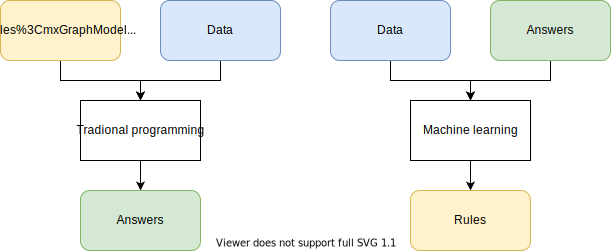
\includegraphics[height=5cm, keepaspectratio]{programming_paradigm_shift.png}
    \caption{A fundamental shift in how we think about programming \cite[p. 5f.]{moroney_ai_2020}}
    \label{programming_paradigm_shift}
\end{figure}

In machine learning we use the answers and the data as input to the development process and the rules are the output we produce. Figure \ref{programming_paradigm_shift} contrasts this change in programming.

Consider any linear function of the form:
$$
    f(x) = w_1x + w_0,
$$
with $ x, w_1, w_0 \in \mathbb{R} $. We could use this function to make predictions about one dimensional input data. For example we might have the living space of houses in $ m^2 $ $ X_i $ and their corresponding price $ Y_i $. We could choose the bias $ w_0 $ and the \textit{weight} $ w_1 $ such that the squared error for the given data is minimal in a process we know as linear regression. When given new data our linear model can make predictions of the potential prices of the houses.


\begin{figure}
    \centering
    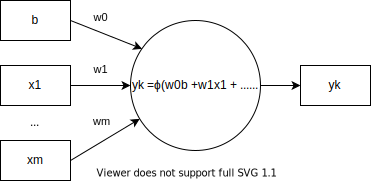
\includegraphics[height=4cm, keepaspectratio]{neural_networks.png}
    \caption{The fundamental idea behind neurons}
    \label{neural_network}
\end{figure}

\begin{figure}
    \centering
    \includegraphics[height=3cm, keepaspectratio]{neural_network_layers.png}
    \caption{A small neural network arranged in layers. An input layer, a hidden layer and an output layer}
    \label{neural_network_layers}
\end{figure}

\paragraph{Activation function}
In this context we refer to such linear functions as \textit{neuron}. An important component is not only the linear function but also the activation function: Before we pass the value of the function f(x) on, we apply some function $ \phi $. The activation function allows us to introduce a non-linearity, which in turn makes smaller networks able to perform much better on more complex tasks than just a simple linear activation. Common functions used are:
\begin{itemize}
    \item ReLu: $ \phi : max(0, f(x)) $
    \item Sigmoid: $ \phi : \frac{1}{1 + e^{f(x)}} $
    \item Binary step: $ \phi : \begin{cases}
                  0 & f(x) < 0    \\
                  1 & f(x) \geq 0 \\
              \end{cases}$
\end{itemize}

This resulting basic neuron is depicted in figure \ref{neural_network}. If we want to make more complex inferences than just the prices of houses, we can arrange multiple neurons into larger structures like chains or layers (\ref{neural_network_layers}). To build such networks we need to generalize the linear function of the neuron for higher dimensional input:

$$
    y_k = \phi\left(\sum_{j=0}^{m}w_jx_j\right)
$$

But this poses a problem. We can find globally optimal solutions with linear regression and the like, but as the size of the network grows, the computational cost of these methods grows too large. A different approach is necessary.

\paragraph{Loss functions} In the context of linear regression the term \textit{mean squared error} was already mentioned. It is the average squared difference between the predictions and the desired output:

$$
    MSE = \frac{1}{n} \sum_{i = 1}^{n}(X_i - Y_i)^2
$$

This is one type of \textit{loss function}, which in general is a measure to describe the error we seek to \textit{minimize} in an optimization process.

\begin{figure}
    \centering
    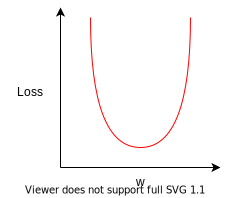
\includegraphics[height=5cm, keepaspectratio]{loss_curve.png}
    \caption{(a) Data points of price versus floor space of houses for sale in Berkeley, CA, in July 2009, along with the linear function hypothesis that minimizes squared-error loss: y = 0.232x + 246. (b) Plot of the loss function for various values of $ w_0 $, $ w_1 $. Note that the loss function is convex, with a single global minimum. \cite[p. 1251]{russell_artificial_2021}}
    \label{loss_curve}
\end{figure}

\paragraph{(Stochastic) gradient descent and backpropagation} By utilizing the loss function we can feed an input into the network and measure for any permutation of the weights $ w_i $ how big the error of the network is. By measuring the loss of the training set $ X_i $ we can find out how well the current configuration of the network fits the data.

Let's go back to the problem of house price prediction. If we plot the MSE for the weights $ w_0 $ and $ w_1 $ of our single neuron the result is a parabola in figure \ref{loss_curve}. Ideally, we want to walk down into the valley where the error is minimal. So for any given combination of the weights we have to find out in which direction the downward slope maximal. The direction of the greatest change of a scalar function is called gradient, which is formalized as follows:

$$
    \nabla f(p)=\left[\begin{array}{c}
            \dfrac{\partial f}{\partial x_1}(p) \\
            \dfrac{\partial f}{\partial x_2}(p) \\
            \vdots                              \\
            \dfrac{\partial f}{\partial x_n}(p)
        \end{array}\right]
$$,
where the point $p $ is a point in the \textit{parameter space}, e.g. as depicted in figure \ref{loss_curve}(b) for $w_0 $ and $ w_1 $. For a single neuron we can use the methods learned in calculus to find the respective \textit{partial derivatives} $  \dfrac{\partial f}{\partial x_i}(p) $. By repeatedly calculating the gradient and updating the weights to move further in the direction of the downward slope, we describe the algorithm of gradient descent:

\begin{algorithm}
    \caption{Gradient descent outline \cite[p. 1253]{russell_artificial_2021}}\label{alg:gradient_descent}
    \begin{algorithmic}
        \State $w \gets \text{any point in the parameter space}$
        \While{not converged}
        \ForEach{$w_i$ in $w$}
        \State $w_i \gets w_i - \alpha \dfrac{\partial f}{\partial w_i}(Loss(w))$
        \EndFor
        \EndWhile
    \end{algorithmic}
\end{algorithm}

The variable $ \alpha $ for gradient descent describes the \textit{learning rate}, so by how much we update the weights. The problem is, as soon as we start combining multiple neurons the intuition gained in calculus on how to calculate the gradient breaks down. Luckily our tools still suffice, we just need to inspect the network more closely. Lets constrain our range of possible neural networks by two conditions:

\begin{itemize}
    \item All functions utilized by the neuron and the network (activation, linear combination of weights) have to be differentiable
    \item The network has to be a directed graph, thus, no loops etc.
\end{itemize}

This makes the neural networks one type of \textit{computational graph}, which have the convenient property letting us find the gradients of the weights in respect to the loss by \textit{backpropagation} by essentially applying the chain rule. Figure \ref{computational_graph} shows an example of a computational graph and its derivation.

\begin{figure}[!h]
    \centering
    \subfloat[Functions are nodes]{
        \includegraphics[width=6cm, keepaspectratio]{computational_graph_functions.png}
    }
    % \hfill
    \subfloat[Differentiate the graph by node $e$]{
        \includegraphics[width=6cm, keepaspectratio]{computational_graph_derivative.png}
    }
    \caption{An example of a computational graph}
    \label{computational_graph}
\end{figure}

In summary, by defining a neural network, we define a weight space. This space is essentially a room of all possible permutations of the weights. We can think of neural networks as functions of programs. Thus, the architecture of the neural network decides on a range of possible programs. Each of these programs is more or less suited for the task given. The feedback given by the loss function indicates the suitability. With gradient descent we search this space of programs for one that minimizes the error. Due to the nature of gradient descent, we are not guaranteed to find the globally optimal program.

\subsection{Convolutional Neural Network}
As we've already stated, we are not limited to one particular type of function in the neural network or computational graph as long as the function can be differentiated. As shown in \ref{neural_network_layers} in its basic form, neural networks have a n-dimensional vector as input. If we have an input like an image, we would have to break down the information about the adjacency to fit the form of a vector. As a result, permutations of the values of the image wouldn't change the result of the output.

Furthermore, the computational requirements for such an approach would grow rapidly. A fully connected first layer would need $n^2$ weights for an image of the size $n$. A small image of the size 256x256 would need 65536 weights for the first layer alone. Ideally we would also like the output of the network to be invariant to translation. This means that a pattern found in the corner should produce the same response as a pattern found in the center of the image.

To achieve this we can utilize convolution. In general terms a "convolution is an integral that expresses the amount of overlap of one function $g$ as it is shifted over another function $f$." \cite{weisstein_convolution_nodate}

$$
    f * g(x) = \int_{-\infty}^{\infty} f(t)g(x - t) dt
$$

This might seem very abstract but firstly, only the discrete case is relevant to us and secondly, only the finite case. This boils down the convolution to filtering $F$, which also comes up in image processing:

$$
    F(u, v) = \sum_{x} \sum_{y} I(u+x, v+y)H(x, y)
$$

For a given coordinate $u,v$ each value in the Kernel $H$ is multiplied by the  corresponding value of the image returned by function $I$. The figure \ref{convolution} illustrates how a convolution would look on a black and white image. In image processing for example, we might use a Laplacian filter to extract certain features like edges. By using convolutions in a neural network we move away from these hand-crafted features by letting the parameters of the kernels be trained to fit the desired outcome. By combining multiple layers of convolutions the network can extract higher level abstractions of the image. \cite{ilin_abstraction_2017}

\begin{figure}
    \centering
    \includegraphics[height=5cm, keepaspectratio]{convolution.png}
    \caption{Convolution of a 8x8 black and white image with a 3x3 kernel, no padding and a stride of 1. \cite{bruasdal_deep_2020}}
    \label{convolution}
\end{figure}


The application of this method for image related tasks has become very popular. The first large scale application in 2012 by Krizhevsky et al. \cite{krizhevsky_imagenet_2017} vastly outperformed any previous methods. This approach is very relevant to the board game setting in Abalone as each board position is essentially an image. Patterns of marbles are relevant in different positions of the board just as different shapes and objects in different places in an image.

\subsection{Residual networks}
By stacking many layers a network can fit more complex domains. Their size has earned them the name deep neural networks. But a central issue with increasing the size of the network is the problem of vanishing gradients.

This section on neural networks has only touched the raw fundamentals of neural networks very swiftly. Nevertheless it shows that the core ideas are quite simple (in hindsight of course), especially compared to the very comprehensive methods of classical AI. The theoretic foundations to these methods are actually quite old. With the unlocking of more and more computational power and data researchers discovered the "unreasonable effectiveness of data \cite{halevy_unreasonable_2009} and the combination of neural networks and gradient descent. To dive deeper the book "Artificial Intelligence: A Modern Approach" \cite{russell_artificial_2021} offers a very good first impression.

\subsection{AlphaGo}
Now we have reached the culmination of our theoretical analysis. All the components we introduced so far constitute the knowledge necessary to understand AlphaGo and AlphaZero. Just like Abalone Go is a perfect information zero-sum board game. It already popped up in the complexity comparison \ref{complexity_table}, which clearly shows, that Go is more complex in its state space and its search tree. At the time when there was a lot of success in other games with minimax many people saw Go as the most challenging board game \cite{muller_computer_2002}. The only successful method at the time was MCTS, for which we already saw two influential papers in the context of Go and MCTS by David Silver.

By combining the reinforcement learning framework with MCTS and neural networks David Silver et al. achieved the milestone of beating Lee Seedol. The program AlphaGo consists of three key components:

\begin{enumerate}
    \item A rollout policy network $p_{\pi}$ and a policy network $p_{\sigma}$ trained by supervised learning
    \item A policy network $p_p$ trained with reinforcement learning and a value network $v_{\theta}$ derived from $p_p$
    \item Lookahead search using (asynchrous) Monte Carlo Tree Search guided by $p_{\sigma}$ and $v_{\theta}$. The rollouts for the search are performed by the rollout network $p_{\pi}$.
\end{enumerate}

The first step is the supervised training based on the KGS Go Server dataset of 30 million positions. The rollout policy network $p_{\pi}$ is a relatively small network that is supposed to provide quick rollouts (simulations). As we already encountered for Abalone this is necessary because random rollouts for such complex games can produce very weak guidance for low numbers and also very long matches. This is supported by comparisons made between the prediction quality of 100 rollouts with a uniformly random policy versus with the network $p_{\pi}$ in figure \ref{alpha_go_prediction_quality}.

\begin{figure}
    \centering
    \includegraphics[height=4cm, keepaspectratio]{alpha_go_prediction_quality.png}
    \caption{Comparision prediction quality of the different components \cite{silver_mastering_2016}}
    \label{alpha_go_prediction_quality}
\end{figure}

The policy network $p_{\sigma}$ is trained in the same fashion except it is larger is size and thus is computationally more expensive. This network is used for the next step in which the network $p_{p}$ is initialized with equivalent structure and weights. We then start to play games with the current version of the policy network $p_{p}$ against random previous versions of the network. At timestep $t$, for a mini-batch of $n$ games, the results of the games are taken and gradient ascent is used to fit the weights to the outcome of the game $z_t$.

$$
    \nabla p \propto \frac{\partial \log p_p(a_t \mid s_t)}{\partial p}z_t
$$

This is the core of the REINFORCE algorithm. \cite{williams_simple_nodate}
\begin{figure}
    \centering
    \includegraphics[height=6cm, keepaspectratio]{alpha_go_mcts.png}
    \caption{Monte Carlo Tree Search in AlphaGo. \cite{silver_mastering_2016} Note the algorithm structure mentioned in figure \ref{monte_carlo_tree_search} is maintained, but selection and simulation is more advanced}
    \label{alpha_go_mcts}
\end{figure}

A more detailed entry to the topic is provided by the nature article "Mastering the game of Go with deep neural networks and tree search". \cite{silver_mastering_2016}

\subsection{AlphaZero}
A problem with AlphaGo's architecture is it's complexity. There are many hyperparameters for the four different neural networks and many other moving parts. AlphaZero is a simplification that conveniently performs much better and is easier to generalize.

\section{Abalone}
Abalone was devised Michel Lalet and Laurent Lévi. Even though it was created fairly recently more than four million global sales have established Abalone as a classic game \cite{noauthor_abalone_2020}.

\subsection{Rules}

\begin{figure}[!h]
    \centering
    \subfloat[Starting position]{
        \includegraphics[width=4.5cm, keepaspectratio]{rules_starting_position.png}
    }
    \hfill
    \subfloat["In-line" moves]{
        \includegraphics[width=4.5cm, keepaspectratio]{rules_inline_move.png}
    }
    \hfill
    \subfloat["Side-step" moves]{
        \includegraphics[width=4.5cm, keepaspectratio]{rules_side_step_move.png}
    }
    \caption{Basic moves \cite{abalone_sa_abalone_nodate}}
    \label{basics}
\end{figure}

In the classical variant each player places 14 marbles on opposing sides. The game's starting position is depicted in figure \ref{basics} (a). There are also other starting position like "German daisy" and "Belgian daisy", as well as four player variants, which will not be considered. One, two, or three adjacent marbles (of the player's own color) may be moved in one of the six possible directions during a player's turn. The marbles have to move in the same direction and can only move to a neighboring field. We differentiate between broadside or "side-step" moves and "in-line" moves, depending on how the chain of marbles moves relative to its direction. The difference is shown in figure \ref{basics} (b) and (c).

\begin{figure}[!h]
    \centering
    \subfloat["2-push-1" sumito]{
        \includegraphics[width=4.5cm, keepaspectratio]{rules_2-push-1_sumito.png}
    }
    \hfill
    \subfloat["3-push-1" sumito]{
        \includegraphics[width=4.5cm, keepaspectratio]{rules_3-push-1_sumito.png}
    }
    \hfill
    \subfloat["3-push-2" sumito]{
        \includegraphics[width=4.5cm, keepaspectratio]{rules_3-push-2_sumito.png}
    }
    \caption{Sumito positions allow pushing the opponent's marbles \cite{abalone_sa_abalone_nodate}}
    \label{sumito}
\end{figure}

A move pushing the opponent's marbles is called "sumito" and comes in three variations, as shown by figure \ref{sumito}. Essentially, the player has to push with superior numbers and the opponent's marbles can not be blocked.

\begin{figure}[!h]
    \centering
    \subfloat[Different blocking situations]{
        \includegraphics[width=4.5cm, keepaspectratio]{rules_block.png}
    }
    \hfill
    \subfloat[Attacking position]{
        \includegraphics[width=4.5cm, keepaspectratio]{rules_attacking_move.png}
    }
    \hfill
    \subfloat[No legal move available to black]{
        \includegraphics[width=4.5cm, keepaspectratio]{rules_stalemate.png}
    }
    \caption{Additional relevant board positions \cite{abalone_sa_abalone_nodate}}
    \label{additional_relevant_positions}
\end{figure}

The figure \ref{additional_relevant_positions} (a) shows ways in which a sumito might be blocked. In 1) the sumito by black is blocked by the black marble, in 2) there is a free space between the marbles and 3) shows how a side-step cannot push a marble. Sumito moves are the only moves that allow for pushing the enemie's marbles, therefore they are the only attacking moves. Figure \ref{additional_relevant_positions} (b) shows a situation in which we can push an enemies marble from the board. The player that pushes six of the opponent's marbles from the board has won. The basic ruleset does not account for a draws but there are, in theory, positions like a stalemate in chess, where no move is possible for one player. In figure \ref{additional_relevant_positions} (c) the black player is locked to the brink of the board and has no move available. Moreover, to force a more eventful game games are often eitherlimited by time or by number of moves. Thus, a draw might occurr when the number of marbles left on the board is equal for each player.

\subsection{Task environment}
Based on the PEAS framework we can specify Abalone as a task environment and show the key components for the implementation of our agent. \cite[p.107]{russell_artificial_2021}

\begin{description}
    \item[Performance measure] Win/loss, number of moves, time to deliberate
    \item[Environment] Digital playing board and rules of the game
    \item[Actuators] Move marbles
    \item[Sensors] Position of marbles
\end{description}

Using the environment properties learned in \ref{environment} we can classify Abalone as \textbf{a fully observable, deterministic, two-agent, competitive, sequential, static and discrete environment}. Another popular term for this type of environment is a \textit{deterministic two-player  turn-based perfect information zero-sum game}.

\subsection{Complexity}
As Abalone has a finite amount of discrete states, we can make precise statements about its complexity, which can be described in two relevant dimensions.

\paragraph{State space complexity}
The state space is the set of all possible states "the environment can be in".\cite[p. 150]{russell_artificial_2021} For Abalone this means we have to consider all possible board configurations with different numbers of marbles present. Additionally, we would have to remove duplicates that arise from the symmetries of the board. In the case of abalone we have 6 rotations and 6 axes we can mirror the board on. The following formula gives us a good upper bound:

\begin{equation}
    \sum_{k=8}^{14}\sum_{m=9}^{14}\frac{61!}{k!(61-k)!}\times\frac{(61-k)!}{m!((61-k)-m)!}
\end{equation}

As the board has six rotational symmetries and additional six mirror axis we have to divide the result by 12 which results in a total of $ 6 \times 10^{23} $ possible board configurations. \cite[p. 4]{lemmens_constructing_2005}

\paragraph{Game tree complexity} The game tree contains all possible transitions between board positions (nodes) through moves (edges). The root of the tree is the default start position. The \textit{search tree} is potentially a subset of the game tree, if not all paths are visited. In the case of Abalone the game tree is unbound and has an infinite height as actions might be taken repeatedly forming loops. Therefore, Abalone's complexity can only be approximateed by an average search tree not the game tree. First we consider the branching factor $ b $, or the number of possible moves for any given state. This number greatly varies between different states. On average Abalone has $ b = 60 $ possible moves per state as measured in figure \ref{branching_factor}. The depth $ d $ of the tree depends on the number of turns per game. Looking at the average again a game takes in the region of $ d = 87 $ turns. To get a measure of the complexity the number of nodes in a tree is given by

\begin{equation}
    b^d
\end{equation}

resulting in a total of $60^{87} \approx 5 \times 10^{154}$ nodes. \cite{lemmens_constructing_2005}

\begin{figure}
    \centering
    \includegraphics[width=7cm, keepaspectratio]{distribution_of_moves.png}
    \caption{Counts of moves available a random player in 5 games}
    \label{branching_factor}
\end{figure}

As those numbers in isolation are hard to grasp it is useful to put Abalone's complexity in relation with other popular games. Its state space complexity is on the same level as Reversi, whilst its game tree surpasses chess in complexity (c.f. table \ref{complexity_table})

\begin{table}
    \begin{center}
        \begin{tabular}{ | c | c | c | }
            \hline
            Game        & state-space complexity (log) & game-tree complexity (log) \\
            \hline
            Tic-tac-toe & 3                            & 5                          \\
            \hline
            Reversi     & 28                           & 58                         \\
            \hline
            Chess       & 46                           & 123                        \\
            \hline
            Abalone     & 24                           & 154                        \\
            \hline
            Go          & 172                          & 360                        \\
            \hline
        \end{tabular}
    \end{center}
    \caption{Abalone in comparison with other games \cite{chorus_implementing_2009}}
    \label{complexity_table}
\end{table}

\subsection{Existing game playing agents}
For all the previously discussed methods, game-playing agents based on minimax have been the most successful so far. Heuristic functions are quite similar to those mentioned for chess. Some of the more significant game situations optimized for are:

\begin{itemize}
    \item Adjacency: As a majority of marbles is required to push the opponent's marbles and conversely an equal amount of marbles is needed to avoid being pushed, it can be assumed that keeping one's marbles grouped together is a good move.
    \item Distance to center: Marbles that are close to the brink of the board put them into danger of being attacked, wherefore it is generally good to place all of the marbles into the center of the board. For each player's marbles we measure their distance from the center of the board as the smallest amount of moves it would take to reach the center (Manhattan distance).
    \item Number of marbles, formation break, single and double marble capturing danger, ... \cite[p. 64]{papadopoulos_exploring_2012}
\end{itemize}

There are multiple implementations of minimax for Abalone \cite{chorus_implementing_2009,lemmens_constructing_2005,ozcan_simple_2004-1,aichholzer_algorithmic_2002}, but only for ABA-PRO by Tino Werner from 2002 there is software openly available \cite{aichholzer_oswin_2006}.  There are a few mentions of (commercial) Abalone programs like RandomAba (Random Soft), AliAba, AbaloneNet mentioned by Lemmens \cite[p. 7]{lemmens_constructing_2005} but those have not been attainable through the internet. Aside from previously mentioned optimizations for minimax like alpha-beta pruning these programs use more advanced techniques like quiescence search, aspiration windows and combined move ordering. A more recent publication from 2012 by Papadopoulos et. al. claimed to have devised a more successful player. \cite{papadopoulos_exploring_2012}  Those claims could not be confirmed entirely in a recent reimplementation thesis by Michiel Verloop as the paper does not describe the weights for the heuristic \cite{verloop_critical_nodate}. This reimplementation in Java \cite{verloop_abaloneai_nodate} is also the reference for later benchmarks as it is open source. \cite{verloop_abaloneai_nodate}

The investigations into MCTS in the context of Abalone are quite limited so far. Pascal Chorus has undertaken a comparison of the vanilla implementation against a heuristic agent, showing the dominance of the heuristic agent. \cite{chorus_implementing_2009} While in games like Go we don't have loops in Abalone, random players can get stuck in very long games making the results of simulations very weak signals. Without any more sophisticated rollout-policy this approach does not work very well.

"Abalearn" was the first learning-based approach to playing Abalone. \cite{campos_abalearn_2003} It was created in 2003 based on temporal difference learning (TD-learning), which is a reinforcement learning method. In the years before TD-learning had been very successful for backgammon ("TD-Gammon") \cite{tesauro_td-gammon_1994} and for Abalone the authors achieved to draw ABA-PRO up to a search depth of five. An interesting feature of their approach is the fact that they exclusively used self-play for training the algorithm. Moreover, they introduced a tunable mechanism for making the risk sensitivity of the algorithm dealing with proplem of the agent playing very passively or getting stuck in loops. Modern reinforcement learning methods like Q-learning have only been considered in a smaller project that achieved better than random performance. \cite{mizrachi_introduction_2017}